\documentclass{article}

\usepackage{xeCJK}
\usepackage{listings}
\usepackage{amsmath}
\usepackage{indentfirst}
\usepackage{graphicx}

\setlength{\parindent}{2em}
\usepackage[colorlinks, urlcolor=blue]{hyperref}
\usepackage[a4paper, left = 2cm, right = 2cm]{geometry}

\begin{document}

\begin{titlepage}
    \title{PTM: pre-trained model}
    \author{\href{https://github.com/ZacBi}{Zac Bi}}
    \date{\today}
    \maketitle
    \pagestyle{empty}
\end{titlepage}

\section{PTM}

最近看这篇综述\href{http://arxiv.org/abs/2003.08271}{Pre-trained Models for Natural Language Processing: A Survey}, 发现PTM的很多细节没了解, 甚至大部分都没有读过,
这就很成问题了, 加上之前关于Transformer和attention的笔记应为WSL升级全部丢失了, 趁这个机会把预训练模型过一遍.

\subsection{Transformer: attention is all you need}

开坑

\subsection{BERT: bidirectional encoder representation from transformer}

开坑

\subsection{ERNIE}

开坑

\subsection{XLNET}

开坑

\subsection{RoBERTa}

开坑

\subsection{\href{https://arxiv.org/abs/1906.08101}{BERT-wwm: Pre-Training with Whole Word Masking for Chinese BERT}}

\subsubsection{Main idea}

熟读BERT应该知道, BERT中的bidirectional正是通过MLM(masked language model)实现的. 原Paper中的具体做法是在预训练的过程中选择sentence中的15\%的token进行mask,
然后预测这些mask应该表示的真实token, 同时, 为了防止pretrain和finetune的错配, 对于需要mask的token采用用三种方式进行mask: 80\%的情况下mask的token是真的'\textbf{[MASK]}';
10\%的情况下是随机token; 10\%的情况下是真正的token.

BERT MLM 的缺陷在于他是随机对wordpiece进行mask的, WWM的主要贡献在于对\textbf{整个词mask以强迫模型学习词的边界}.
注意BERT-wwm只是对BERT的一个补丁, 而不是创造了一个新的模型.
贴个paper的图片(CWS指的是paper中采用LTP的chinese word segmentation):

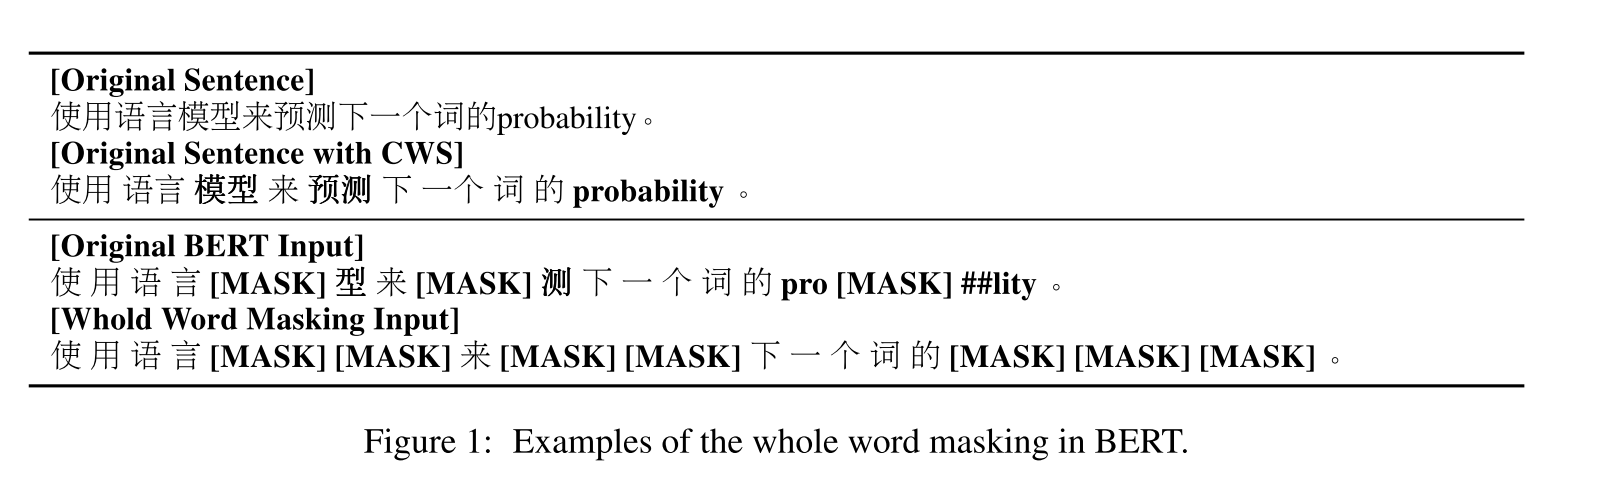
\includegraphics[scale=0.27]{BERT-wmm.png}

\subsubsection{Pre-training details}

上一小节中提到BERT-wwm是对BERT的一个补丁, 所以paper中没有从头开始对BERT进行预训练, 而是直接用BERT的checkpoint再训练.
训练分为两个阶段, 第一个阶段采用长度为128的输入, 目的是\textbf{计算高效性}, 第二阶段采用的长度为512的输入, 目的是\textbf{学习长距离依赖}
(第二阶段的输入不是简单的加入'\textbf{[PAD]}', 而是把raw dataset重新划分长度了). 每一阶段都训练了100k steps.

两步的初始学习率都是1e-4, warmup比例为10\%, BERT-wwm采用optimizer的不是BERT的AdamW而是LAMB(好吧我连AdamW也忘了复习了).
\textbf{最最重要的是BERT-wwm是base模型}, 关于base, large请看BERT原文.

Paper中出现了BERT-wwm-ext, 我在内容里面找了一圈没发现这啥意思, 看了官方的\href{https://github.com/ymcui/Chinese-BERT-wwm}{github repo}才知道,
是增加了语料库的大小, 官方描述是"囊括了百科、问答、新闻等通用语料,总词数达到5.4B, BERT-wwm-ext采用了与BERT以及BERT-wwm一样的模型结构,
同属base模型,由12层Transformers构成。训练第一阶段(最大长度为128)采用的batch size为2560,训练了1M步。训练第二阶段(最大长度为512)采用的batch size为384,训练了400K步。"

\subsubsection{Experiments}

在各种中文数据集上做了测试, 大概的表现是BERT < ERNIE < BERT-wwm < BERT-wwm-ext < RoBERTa-wwm-ext < RoBERTa-wwm-ext-large.
(模型大真好)

\subsubsection{Useful Tips}

上面的实验中, 每个模型在不同数据集中表现略有不同, paper总结了几点:

\begin{itemize}
    \item 学习率很重要
    \item BERT和BERT-wwm的初始学习率可以设置成一样的, 但是ERNIE不行.
    \item 因为BERT和BERT-wwm都是在Wikipedia这样的有良好形式的文本上训练的, 而ERNIE的语料有一部分是网络上抓取的, 更适合口头或者非正式的文本
    (这应该算是domain migration问题?)
    \item 在更长序列上, 比如机器阅读理解或者文档分类这些, 更适合用BERT和BERT-wwm.
    \item 要谨慎考虑领域迁移的问题, 如果task的文本和预训练的文本差别比较大, 建议先在task文本上进行预训练, 再做微调, 这应该算一个trick.
\end{itemize}

\end{document}